\documentclass[12pt, headsepline, a4paper]{scrartcl}
\usepackage{booktabs}
\usepackage{times}
\usepackage{latexsym}
\usepackage[utf8]{inputenc}
\usepackage{mathtools}
\usepackage[dvipsnames,table,xcdraw]{xcolor}
\usepackage{colortbl}
\usepackage[T1]{fontenc}
\usepackage{verbatim}
\usepackage{booktabs} % Allows the use of \toprule, \midrule and \bottomrule in tables
\usepackage{url}
%erlaubt zitierungen ohne eckige Boxen
\usepackage{natbib}
\usepackage{subcaption}
\usepackage{float}
% Packet für Seitenrandabständex und Einstellung für Seitenränder
\usepackage{geometry}
\geometry{left=3cm, right=3cm, top=2.5cm, bottom=1.5cm}


%nointend
\usepackage[parfill]{parskip}

% neue Kopfzeilen mit fancypaket
\usepackage{fancyhdr} %Paket laden
\pagestyle{fancy} %eigener Seitenstil
\fancyhf{} %alle Kopf- und Fußzeilenfelder bereinigen
\fancyhead[L]{\nouppercase{\leftmark}} %Kopfzeile links
\fancyhead[C]{} %zentrierte Kopfzeile
\fancyhead[R]{\thepage} %Kopfzeile rechts
\renewcommand{\headrulewidth}{0.4pt} %obere Trennlinie


\title{Taxonomy refinement using distributional semantics}
\author{Rami Aly \\ Universität Hamburg}


\date{\today}

\begin{document}
\maketitle
\begin{abstract}
As part of the project "Shared Tasks for Natural Language Processing" we propose a method to improve existing domain-specific taxonomies by applying a pipeline of refinement steps. Most notably, we introduce the use of Poincaré embeddings as a solution to identify wrong hypernym relationships within a taxonomy as well as to attach disconnected components to a taxonomy. We applied the proposed method  to all available domains of the SemEval-2016 Task 13 for the English language and obtained state-of-the-arts results with significant improvements.
\end{abstract}

\begin{comment}
	  As part of the project "Shared Tasks for Natural Language Processing" we propose a method to improve existing domain-sepcific taxonomies by a applying a pipeline of refinement steps.  Most notably, we introduce the use of Poincaré embeddings as a solution to attach disconnected components to a taxonomy. We further use the embeddings to identify wrong hypernym relationships within a taxonomy. We applied the proposed method on the SemEval-2016 Task 13 for the English language for three domains (Environment, Science and Food) and obtained state-of-the-arts results with significant improvements.
\end{comment}


\section{Introduction}
The task of taxonomy induction aims to create a semantic hierarchy of entities by hyponym-hypernym relations, called \emph{taxonomy}, from text corpora . It is a useful tool for tasks such as content organization and retrieval. Compared to many other domains of natural language processing that make use of more recent techniques, like word embeddings and deep neural networks, the task of taxonomy learning is still highly reliable on traditional approaches like extraction of lexico-syntactic patterns \citep{Hearst:1992:AAH:992133.992154} or co-ocurrence information \citep{grefenstette2015inriasac}. The use of distributional semantics \citep{mikolov2013distributed} for hypernym identification has received increasing attraction, however, multiple concerns were raised. \cite{levy2015supervised} observe that instead of the relation between the two terms x and y, these methods actually learn the independent attribute of a term to be a so called \emph{prototypical hypernym}. Therefore, although usable for hypernym detection, past applications of distributional semantics appear to be rather unsuitable to be directly applied to taxonomies. 


We address that issue by introducing a pipeline of refinement steps that employ distributional semantics, in order to improve an existing domain-specific taxonomy. The refinement method deals with the most prominent errors of a taxonomy: Wrong relationships between terms as well as completely disconnected elements. In addition to traditional word2vec embeddings we employ domain-specific Poincaré embeddings. We observe that Poincaré embeddings highly outperform traditional word2vec embeddings. We hypothesize that the difference is explained by the incorporation of the hierarchy between terms within Poincaré embeddings. We apply the refinement pipeline to taxonomies that are generated by the taxonomy induction system TAXI \citep{panchenko2016taxi}, which achieved the highest score for the above mentioned shared task and uses a combination of lexico-syntactic patterns and substring matching techniques. Therefore, this refinement technique employs distributional semantics as a complementary method on a taxonomy induction system, that is based on more traditional methods. We designed this refinement method to be applied non-restrictively to any domain and language by solely depending on raw text processing. The techniques are applied to all domains of the shared task for the English language. 


The reimplementation of TAXI was done by Alex Ossa and me together. However, we worked mainly independently on each topic to improve the existing taxonomy. While Alex employed a deep neural network method, called \emph{Hypenet} \citep{shwartz2016improving} and is going to document his part in a separate report, this paper aims to cover the topic of distributional semantics that I dealt with.

\begin{comment}
the ineffectivness is indicated by a submission to the SemEval-2016 Task 13 scoring the lowest using distributional semantics for taxonomy construction \citep{pocostales2016nuig, bordea2016semeval}.


The aim of the project "Shared Task for Natural Language Processing" was to engage students in one of several shared tasks that deal with a specific aspect of natural language processing. We focused on "Taxonomy Extraction" as part of the SemEval-2016 Task 13, with the aim to create a semantic hierarchy of entities by \emph{is-a} relations, called \emph{taxonomy}, on domain-specific entities. We particularly focused on the submission done by \cite{panchenko2016taxi}, which proposes the construction of a Taxonomy by a high scaled approach using lexico-syntactic patterns and substrings. They received the first place for this shared task and thus appeared to be a reasonable starting point. The first part of this work consisted of the reimplementation of the above mentioned approach, as only a part of the system was openly accessible. Secondly, we tried to improve the existing taxonomy by using several approaches, most notably  deep neural-network architecture for hypernym-hyponym extraction, called \emph{Hypenet} \citep{shwartz2016improving} and distributional semantics. This report focuses on the latter approach. We employed distributional semantics through a pipeline of refinement steps and used different distributional representations and algorithms to refine the taxonomy, most notably Poincaŕe embeddings. We follow the concept of using exclusively raw data as a pre refinement method so that this refinement technique can be applied non-restrictively to any domain and language. They are used to identify outliers and attach unconnected entities to the taxonomy. The techniques are applied on three domains:science, food and environment for the English language.
\end{comment}



\section{Related Work}

A taxonomy is generally speaking the classification of entities, things or concepts in a semantic hierarchy. A taxonomy predominantly aims to create a system with relationships, that can be categorized into so-called predications and universally quantified conditionals. While the latter focuses on types, e.g \emph{monkey is a mammal}, predication relationships focus on concrete entities, for example \emph{Einstein is a scientist} \citep{DBLP:journals/computer/Brachman83}. Both relationship types are so called \emph{is-a} relations, in contrast to relations of a meronomy, which organizes entities in parts of a whole by using \emph{has-a} relations. The two entities of a is-a relationship are called hypernym and hyponym, with the first term describing the generic entity and the latter one a specific instance of the entity. Therefore, is-a relationships are asymmetric and transitive, which is why taxonomies are normally hierarchically structured. Phrases that are hyponyms of the same hypernyms are called co-hyponyms, for example \emph{cat} and \emph{dog}, as both could belong to the hypernym \emph{animal} and neither cat nor dog is a hypernym of one another. The shared task focuses on the taxonomies that are created for nouns. Taxonomies based on verb phrases can be created as well, although this is done only sporadically in literature.
Creating taxonomies is highly beneficial in numerous NLP tasks, such as personalized recommendations \cite{zhang2014taxonomy} or question answering \citep{Yang2017technical}.
The typical workflow of a taxonomy construction technique as described in \cite{wang2017short} consists of two parts. Firstly, the extraction of is-a relationships using either pattern-based or more recently distributional methods and secondly, the construction of the taxonomy from is-a relations using incremental learning, clustering or graph-based induction. Finally, a taxonomy cleansing step is described to remove wrong is-a relations by removing cycles and handling entity ambiguity.


The first shared task on taxonomy extraction was conducted as part of the Semeval 2015 Task 17 \citep{task17semeval2015}. The task is concerned with the automatic extraction of taxonomies from text, also called taxonomy induction. The creation of taxonomies based on human compiled resources such as Wikipedia \citep{mahdisoltani2013yago3, suchanek2007yago} tend to score better since it is difficult to extract knowledge exclusively from text \citep{wang2017short}. However, these large taxonomies often lack domain-specific and long-tailed knowledge. The task of taxonomy induction addresses this issue, since the use of free-text allows to create domain-specific taxonomies. Thus, the task of taxonomy induction is receiving increasing interest. Since this task is far from being solved, the conducted shared task aimed to contribute to the research of this topic. The organizers provided the participants with respective terms for each domain, on which the taxonomy should be built upon, because the subtask of \emph{Term extraction} is a relatively well-known task and in order to simplify the evaluation. Therefore, submitted systems take the domain name and the respective terms as an input to induce a domain-specific taxonomy. Six different taxonomy creation systems were submitted. INRIASAC and LT3 reached the first and second positions respectively. The latter system used a web corpus constructed by applying BootCat with the provided domain-specific terms as seed terms. They then extracted relations using lexico-syntactic patterns, morphological structure of compound terms and WordNet lookup. INRIASAC also used lexico-syntactic patterns in addition to substring matching and co-occurrence information to extract relationships of the input domain terms on the basis of a corpus from Wikipedia. 

The second run of this shared task \citep{bordea2016semeval} was extended to a multilingual setting, covering English, French, Italian and Dutch. Moreover, participants were provided with a Wikipedia-based text corpus which was allowed to be manually extended by participants. Five different systems were submitted that year. The second best system, QASSIT \citep{S16-1205} uses a semi-supervised approach and genetic algorithms. They first calculate the similarity between concepts using semantic vectors and then define a pretopology space from which a taxonomy structure is defined. Finally a genetic algorithm is applied to optimize two parameters: the quality of the added relationships in the taxonomy and the quality of its structure.

The best result for SemEval-2016 Task 13 was achieved by a taxonomy induction system called TAXI, that harvests hypernyms with substring inclusion and Hearst-style lexico-syntactic patterns from domain-specific texts, obtained via language model based focused crawling \citep{panchenko2016taxi}. Their doctrine is that taxonomy induction should be driven solely on the basis of raw text processing so that a taxonomy can be introduced in a new domain or a new language for which pre-annotated resourced do not exist. Later, we use the extracted taxonomies generated by their method as a baseline system which is then improved by the refinement pipeline.
Most submissions of the shared task used traditional pattern-based approaches. An exception is the submission by \cite{pocostales2016nuig}, who applied distributional semantics to construct taxonomies. However, their system scored the lowest out of all submissions \citep{bordea2016semeval}.


More refined taxonomy induction systems that apply distributional semantics have been introduced since the second shared task was hold. Most recently, \cite{Zhang:2018:TUT:3219819.3220064} represent each term as a conceptual topic and defines it as a cluster of semantically coherent concept terms. The topic taxonomy is constructed by using term embeddings and hierarchical clustering, recursively for underlying terms. They further include an adaptive spherical clustering module and a local embedding module to maintain the quality of the recursive process. An expressed limitation is that the number of clusters is a hyperparameter that needs to be pre-specified for the recursive process - thus the number of children for each parent is statically defined.

The task of taxonomy creation offers many unsolved challenges. \cite{wang2017short} recommend to study the combination of pattern-based and distributional methods and how they reinforce each other. Besides \cite{shwartz2016improving}, there have been very few approaches that use deep learning paradigms, since it is difficult to design a single objective for neural networks to optimize the task. Finally, the task is also insufficiently studied regarding taxonomies for specific domains and under-resourced languages \citep{wang2017short}. Domain knowledge is essential for relation extraction but difficult to obtain. The taxonomy creation should focus on constructing a taxonomy based on knowledge of a specific domain, as it is especially difficult to develop a "one-size-fits-all" taxonomy. Furthermore, domain taxonomies have a higher coverage than existing methods \citep{alfarone2015unsupervised}.

Our refinement method addresses some of the above mentioned issues by complementary applying a method using domain-specific distributional semantics to a text induced taxonomy, that is based on traditional pattern-based methods. 


\section{TAXI}

\label{TAXI}

The first step of our work consisted in reimplementing TAXI and evaluating some key quantitative statistics. Their method uses a combination of lexico-syntactic pattern and substring matching evaluation on large-scaled domain-specific texts. They take the domain-specific input terms that are provided by the shared task and apply four steps in order to create the taxonomy. 

The first source of candidate hypernyms is attained by substring matching. In this method, a substring score is calculated for each input term $\sigma(t_i, t_j) = \frac{length(t_j)}{length(t_i)}$ with $t_i$ being the hypernym term and $tj$ the hyponym term. If we find the same compound word in reverse order, the substring score will be set to zero.  If $\sigma(t_i, t_j)$ is larger than three, the relation will be added as a candidate. 

The next source of hypernyms is the use of lexico-syntactic patterns. For this purpose, general corpora and domain-specific corpora are crawled based on the input terms.  In order to achieve this, general corpora of Wikipedia, CommonCrawl and about 59.2GB of data extracted from English Wikipedia, Gigaword \citep{parker} ukWac \citep{Ferraresi} and a news corpora from the Leipzig Collection \citep{goldhahn} are collected. The domain-specific corpora consist of web pages that have been selected by using a combination of BootCat and focused crawling \citep{remus2016domain}. Bootcat collects the URLs, that return after sending predefined terms to a Web search engine. These URLs are then used as the seed for a focused crawling method to create a larger corpus of domain-specific web pages. 
Then multiple systems are applied(PattaMaika \citep{kluegl2016uima}, PatternSim \citep{konvens:23_panchenko12p}, and \mbox{WebISA} \citep{Seitner2016ALD}), which all use lexico-syntactic patterns, such as the ones described by \cite{Hearst:1992:AAH:992133.992154}. Patterns like \emph{NP$_0$ , including NP (... and/or NP)}, with NP$_0$ being the hypernym and NP the hyponym are used to extract noisy is-a relations from the general and domain-specific corpora. Since the extracted hypernyms based on lexico-syntactic contain many noisy relations, an asymmetric pattern-based hypernymy score $\pi(t_i, t_j)$ was introduced. This score combines the information  from different hypernym collections and is computed by $\pi^k(t_i, t_j) = \frac{freq^k(t_o, t_j)}{max_jfreq^k(t_i, t_j)}$ for the k-th extractor and with $freq^k(t_i,t_j)$ being the frequency of relations between two terms.


The penultimate step consists of combining the scores of hypernym candidates, extracted by the two aforementioned methods. The work proposes two approaches for this step. The first one is a supervised approach, which trains a classifier on the trial dataset provided with the task. It uses two features, namely $\sigma(t_i, t_j)$ and $\pi(t_i, t_j)$. The second method is a static selection of is-a relations. It keeps all hypernyms extracted by substrings ($\sigma(t_i, t_j) > 0)$ and up to two hypernyms extracted by patterns. Although the original paper uses the supervised approach for the English language, we decided to apply the latter approach for our work. This has several reasons; first of all, using the supervised approach requires training data which is not necessarily available for every domain and language (TAXI uses the supervised approach exclusively for English since trial data was only provided for this language). It thus contradicts the initial idea of creating a taxonomy solely on the basis of raw text processing. Secondly, we had difficulties achieving results comparable to the ones in the paper using the supervised approach, although the important parts of their method are openly accessible\footnote{\url{https://github.com/tudarmstadt-lt/taxi}}.


The last step consisted of pruning and cleaning the noisy taxonomy. This step needed to be re-implemented by us. To identify cycles in the taxonomy, we employed the Tarjan algorithm \citep{tarjan1972depth}. If a cycle is detected, one relation will be removed at random. However, in practice at most two relationships were removed for all domains. That is why we decided, that this simplistic approach is sufficient for most cases. Moreover, we attached all unconnected components to the root (this does not include single disconnected nodes). Lastly, we remove all relationships that have the domain root as a direct or indirect hyponym. Thus, we make sure that the domain root is also the root of the created taxonomy. This step is now part of the official TAXI github, after we made a pull request to include that implementation.

Altogether, the displayed results for the baseline method differ slightly from the original paper for the food and science domain and quite substantially for the environment domain, with our results being worse. The results of the reimplementation and the original TAXI results are listed in Table \ref{baseline} for all three domains (environment, science, food) of the shared task.


\begin{table}
	\begin{tabular}{l | l | c | c | c | c }
		\textbf{System}
		& \textbf{Domain}
		& \textbf{R}
		& \textbf{P}
		& \textbf{F1}
		& \textbf{F\&{}M} \\
		\toprule
		Original TAXI   
		& Environment
		& 0.2682	
		& 0.3382
		& 0.2992	
		& 0.2384
		\\
		Reimplementation   
		& Environment
		& 0.2184	
		& 0.3098
		& 0.2562
		& 0.2489
		\\
		\hline
		Original TAXI   
		& Science
		& 0.3484
		& 0.3876
		& 0.3669
		& 0.3634\\
		Reimplementation    
		& Science
		& 0.3269
		& 0.4164
		& 0.3663
		& 0.3939
		\\\hline
		Original TAXI   
		& Food
		& 0.2376
		& 0.3372
		& 0.2787
		& 0.2021
		\\
		Reimplementation 
		& Food
		& 0.2187
		& 0.3656
		& 0.2736
		& 0.1936
		\\\bottomrule
	\end{tabular}
	\caption{Result comparison between original TAXI and our reimplementation baseline.}
	\label{baseline}
\end{table}

We further evaluated the contribution of the two methods(substring matching and lexico-syntactic patterns) to the total score for the science domain by only executing one of the methods at a time and by comparing the scores. The method using substring matching achieved a score of 0.268 while the pattern matching approach scored 0.11. Therefore, both approaches significantly improve the score although substring matching appears to be the more effective method. We further notice that both methods complement each other very well, as the score using both approaches is very similar to the sum of using them separately.


\section{Taxonomy Refinement Method}
The proposed method uses the existing taxonomy created by the TAXI system, its corresponding domain terms and raw-text corpora to create an improved version of the input taxonomy. The structure of the taxonomy is not restricted, it can be connected or consists of cycles and completely disconnected domain terms. We apply a pipeline of three steps, two of which directly impact the existing taxonomy. The main focus of our refinement method is the use of distributional semantics, in particular Poincaré embeddings. By using them we aim to deal with the most prominent errors of a taxonomy: wrong relationships between terms as well as completely disconnected elements.
The first step consists of creating domain-specific Poincaré embeddings (Section \ref{Poincare_step}). The trained embeddings are then used to identify wrong hypernym relationships in the taxonomy  as well as to attach unconnected terms to the taxonomy (Section \ref{dist_semantics}). In the last step, we further optimize the taxonomy, remove cycles and attach remaining disconnected terms to the root (Section \ref{Improved_Taxonomy}).

\begin{figure*}[tp]
	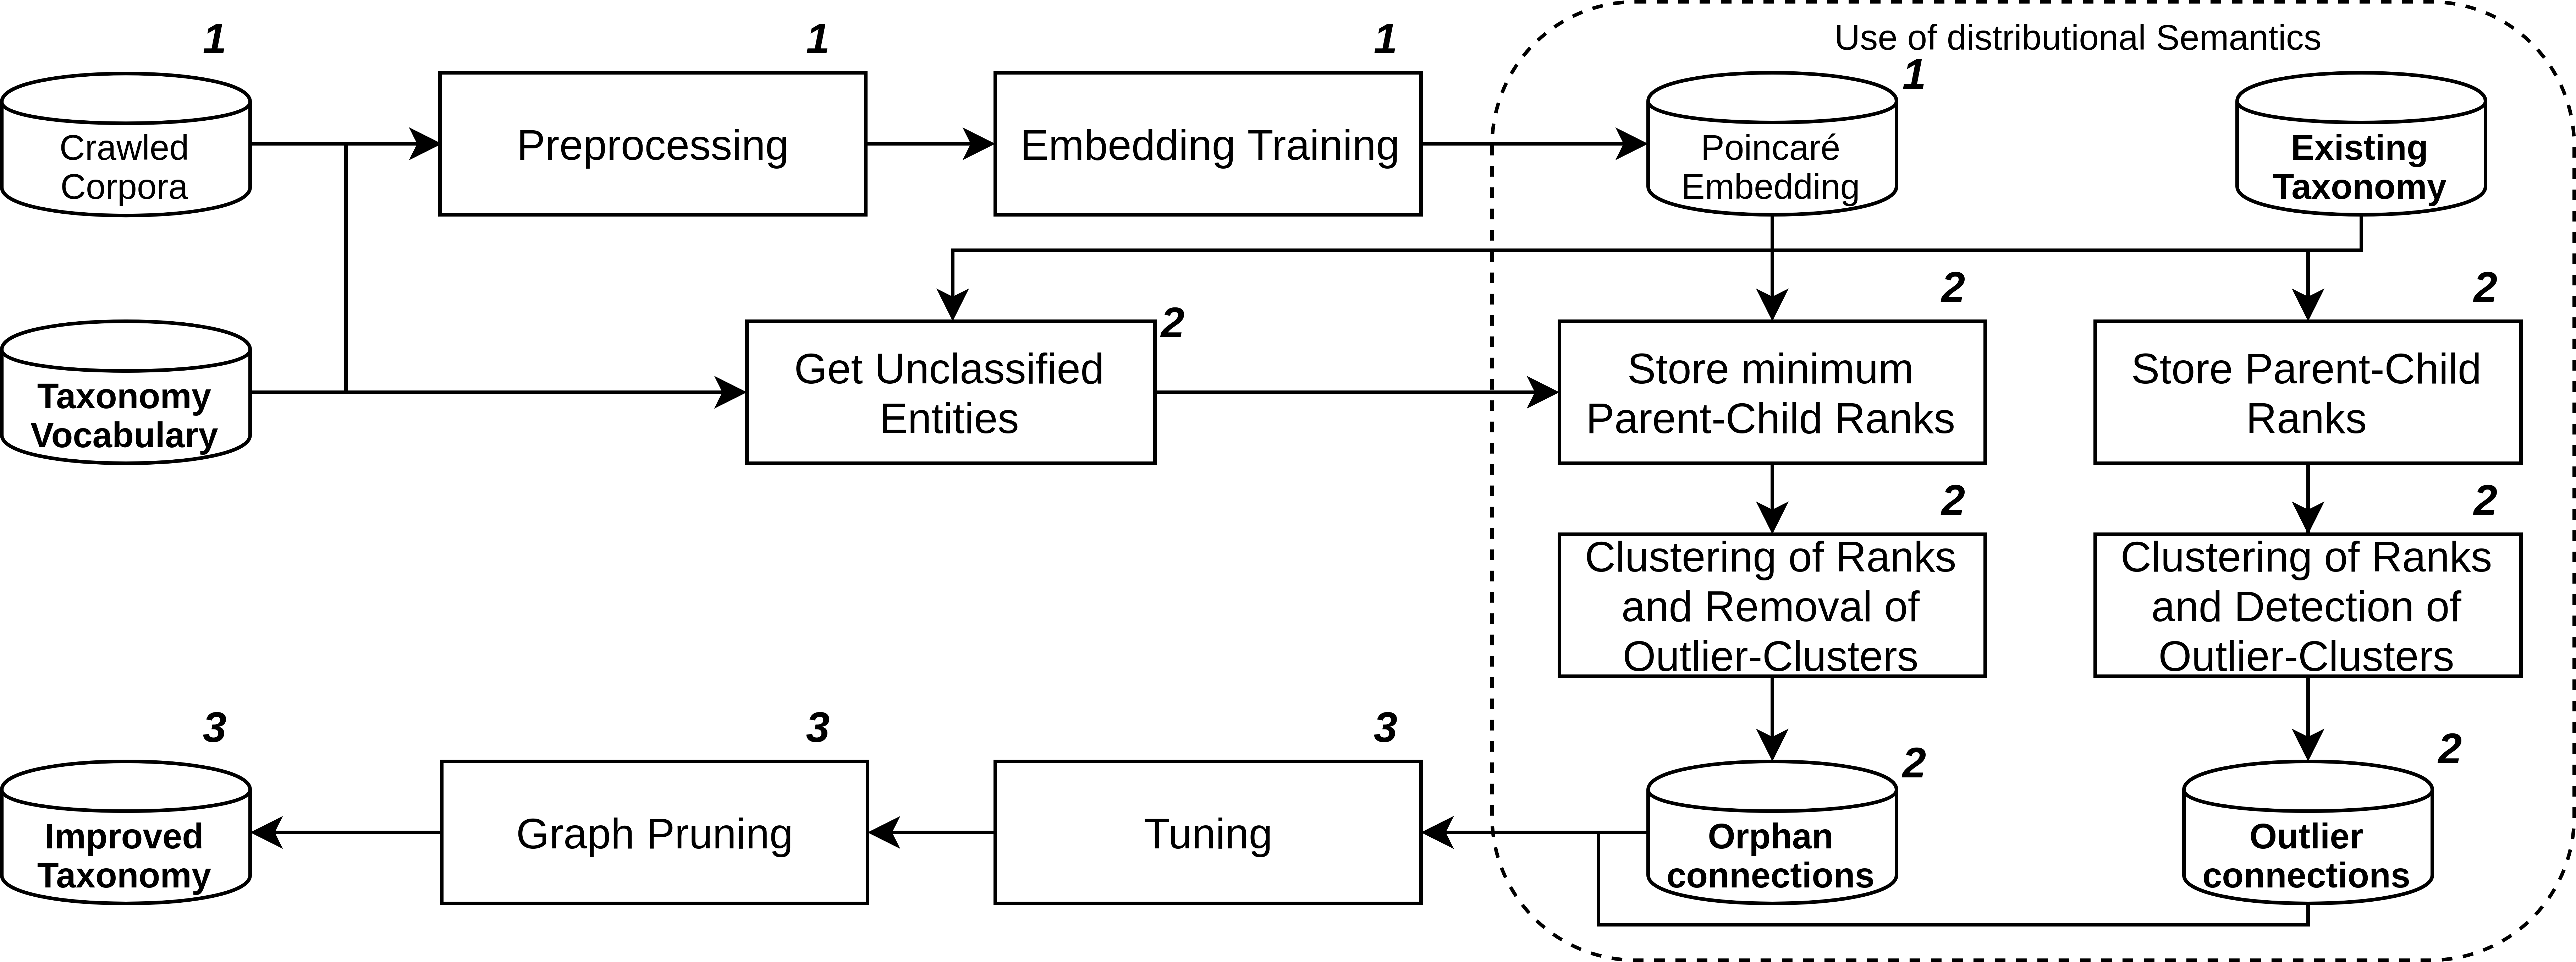
\includegraphics[width=1\textwidth]{images/process_chart7.png}
	\caption{Outline of the underlying process to improve an existing taxonomy. The numbers correspond to the step within the pipeline.}
	\label{process_chart}
\end{figure*}




\subsection{Domain-specific Poincaré Embedding}
\label{Poincare_step}

We aim to construct Poincaré embeddings that are designed for the specific domain of the taxonomy, since using task-specific embeddings have been shown to be more effective than general-purpose embeddings \citep{Li2016JointEO, wang2017short}.
To create suitable Poincaré embeddings we use noisy hypernym relationships, extracted from a combination of general and domain-specific corpora, comparable to the is-a relationships extracted by TAXI. The extracted domain-specific relationships are further filtered to create more accurate but still noisy relationships.

\begin{comment}
As for the general corpora, we use about 59.2GB of data extracted from English Wikipedia, Gigaword \citep{parker} ukWac \citep{Ferraresi} and a news corpora from the Leipzig Collection \citep{goldhahn}. The domain-specific corpora consists of web pages that have been selected by using a combination of BootCat and focused crawling\citep{remus2016domain}. Bootcat collects the URLs, that return after sending predefined terms to a Web search engine. These URLs are then used as the seed for a  focused crawling method to create a larger corpus of domain-specific web pages. 
We then apply multiple systems (PattaMaika \cite{kluegl2016uima}, PatternSim \cite{konvens:23_panchenko12p}, and \mbox{WebISA} \cite{Seitner2016ALD}) which all use lexico-syntactic patterns, such as the ones described by \citep{Hearst:1992:AAH:992133.992154} to extract noisy is-a relations from the extracted general and domain-specific corpora.
\end{comment}

\paragraph{Cleaning} For the next step, the extracted noisy relationships of the common and domain-specific corpora are further processed separately and combined afterwards. 
Let $V$ be the set of all domain terms of a given taxonomy. In order to limit the amount of words and relationships the Poincaré embeddings have to learn, we decide to limit the is-a relationships $R$ on pairs for which both entities are part of the taxonomy's vocabulary. By using only vocabulary of the domain-specific taxonomy, the thus created collection of relationships is domain-specific as well.
Furthermore, every relationship is removed, which is not above a fixed frequency threshold $T_{f}$. 
We further remove every reflexive relationship, so that $ \forall a \in V:(a,a)\not\in R$ holds true. We could include symmetric relationships, however since $R$ is relatively noisy, we decided on only keeping the more frequent pair so that $\forall (a,b) \in R : (f(a,b) - f(b,a)) > T_{f}$ is fulfilled, with $f$ being a function that maps the a pair to the number of occurrences in the collection of extracted relationships. Hence, $R$ is transformed to being antisymmetric and irreflexive. 
Same procedure is applied to all relationships extracted by the common-crawl corpora which are then added to $R$. However, a is-a relation is only added if it does not contradict the properties of $R$, resulting in a collection of relationships in which relationships gathered by common-crawl corpora can only expand but not change $R$ as created by the domain-specific corpora.

\paragraph{Training} These cleaned is-a relationships are then used to train Poincaré embeddings. We choose a dimensionality of 50 and 400 epochs to ensure convergence. We trained an additional model on noun pairs extracted from Wordnet\footnote{https://wordnet.princeton.edu/}. Finally, we also trained word2vec embeddings \citep{mikolov2013distributed} on a wikipedia corpus (Table \ref{hyperparameters}), connecting compound words by a character '\emph{\_}' to be able to natively learn distributional semantics for compound words. This appeared to be a more suitable approach for this task, since combining vector representation of subwords has shown to be difficult for combinations such as \emph{signal processing}. The specific hyperparameters for every embedding model are listed in Appendix \ref{hyperparameters}.


\subsection{Distributional Semantics}
\label{dist_semantics}

In contrast to word2vec which is computed  in euclidean space and commonly applies the cosine distance (similarity)
$\frac{\textbf{u} \cdot \textbf{v}}{|\textbf{u}| |\textbf{v}|}$ as a similarity measure,
Poincaré embeddings use a hyperbolic space, specifically the Poincaré Ball. Poincaré embeddings explicitly capture the hierarchy between words in the embedding space and aim to capture hierarchical relationships more efficiently. The distance between two points $\textbf{u},\textbf{v} \in \mathcal{B}^d$ for a d-dimensional Poincaré Ball model is defined as:
\begin{equation}
\label{poin_eq}
    d(\textbf{u}, \textbf{v}) = \textrm{arcosh}(1 + 2 \frac{||\textbf{u} - \textbf{v} ||^2}{(1 - ||\textbf{u}||^2) (1 - ||\textbf{v}||^2)})
\end{equation}

The Poincaré distance as defined in Eq. \ref{poin_eq} enables us to capture the hierarchy and similarity between words simultaneously. The Poincaré distance increases exponentially with the depth of the hierarchy. So while the distance of a leaf node to most other nodes in the hierarchy is very high, nodes on lower level such as the root, have a comparably small distance to all nodes in the hierarchy, as seen in Figure \ref{poincare_properties}c). Thus, a small distance between two nodes is achieved by a combination of similarity between terms and their respective position in the hierarchy.
Naturally, not all terms of a taxonomy are represented in the trained embeddings. During this step we ignored hypernyms for which no distributional representation exists.

\begin{figure}[tp]
	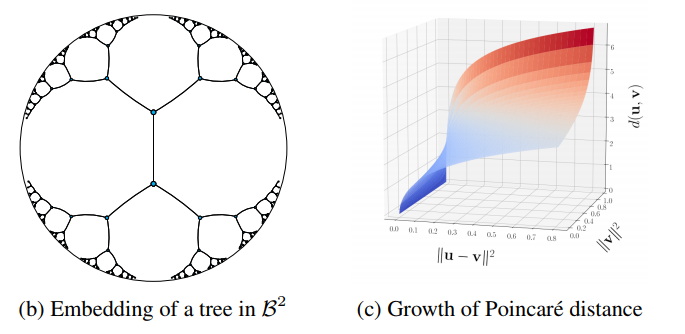
\includegraphics[width=1\textwidth]{images/poincare_properties.png}
	\caption{Visualization of Poincaré embeddings, in b) the length of every edge is of equal length in $\mathcal{B}^2$. c) visualizes the Poincaré distance d(u,v) in relation to the norm $||v||^2$ and the direct distance to another node. Illustration taken from \cite{NIPS2017_7213}}.
	\label{poincare_properties}
\end{figure}


\paragraph{Outlier Identification}
Firstly, we use distributional semantics to detect wrong hypernym relationships in the taxonomy.
The Poincaré embeddings are used to compute a rank between every child and parent of the existing taxonomy. The rank(x,y) is defined as the index of y in the list of all sorted Poincaré distances of all entities to x. In order to detect wrong hypernyms, called \emph{outliers}, we employ k-means on all calculated ranks. The cluster with the highest ranked hypernym is marked. If the cluster is additionally not the center cluster (cluster with most hypernyms) we mark it as an outlier cluster and corresponding relationships are accordingly removed from the taxonomy. This step is repeated until no outlier cluster remains.
The system that uses word2vec aims to find co-hyponym relationships, as word2vec similarity does not capture parent-child relationships. Therefore, we compute the distance to the closest co-hyponym (child of the same parent) for every node. The clustering technique as just introduced is then applied to identify outliers.

\paragraph{Orphan Insertion} 
This step aims to reattach disconnected nodes, called \emph{orphans}, to the respective taxonomy. This includes orphans that were already disconnected in the input taxonomy, as well as orphans that were produced by the removal of relationships in the previous step.
For every term that is not connected to the taxonomy, the parent with the lowest ranked is searched and stored as a potential parent. Similar to aforementioned approach, we apply k-means to the collection of ranks of all potential parents in order to identify the relationships that will be added. All relationships apart from the ones that belong to outlier clusters (if existent) are added to the taxonomy.
The word2vec system applies a similar method. However, the identified relationships are not registered as parent-child relationships but as co-hyponym relationships. Thus, a link is added between the parent of the most similar co-hyponym in the taxonomy and the orphan.

\subsection{Improved Taxonomy}
\label{Improved_Taxonomy}
The final step consists of further improvements of the taxonomy and its structure. In case a distributional representation does not exist for a term, we used a heuristic to determine how to connect an orphan; if a substring of a compound word can be found in the hierarchy, the orphan is linked as a hyponym to that entity. Otherwise, the orphan remains disconnected. This substep depends on the underlying language and possibly needs to be adjusted. All other steps should work independently of language or domain. 

Finally, we repeat the final step of the TAXI system, since the refinement method could theoretically create circles and disconnect components. Thus, we connect disconnected components to the root. We further identify circles again and remove them if detected.


\section{Evaluation}

The proposed methods are evaluated on the SemEval-2016 challenge for Taxonomy Extraction Evaluation \cite{bordea2016semeval}. We evaluate the proposed methods on the English language sub-task.
The baseline taxonomy we refine is the reimplementation of the TAXI system as described in Section \ref{TAXI}.

\paragraph{Metrics} The employed metrics were selected with the goal to exhaustively assess the quality of the taxonomy. 
Quantitative evaluation is done by comparing them against the gold standard of the corresponding domain. The main metrics we employed are recall, $\frac{| E_S \cap{} E_G |}{| E_G |}$, precision $\frac{| E_S \cap{} E_G |}{| E_S |}$, and $F_{1}$ score $\frac{2 * ( P * R )} {( P + R )}$. Additionally, we employed the Fowlkes\&Mallows measure defined in \citep{velardi2013ontolearn, f&m}. It measures how well a taxonomy clusters similar nodes by calculating a score $B_{S,G}^i = \frac{n_{11}^i}{\sqrt{(n_{11}^i + n_{10}^i) \cdot (n_{11}^i + n_{01}^i)}}$ for every cut i in the taxonomy, with $n_{00}$ being the number of object pairs that are in different clusters in the target taxonomy S as well as the gold standard taxonomy G and in same clusters for $n_{11}$. $n_{10}$ and $n_{01}$ are pairs that are in the same cluster in the target taxonomy but not in the gold taxonomy and vice versa.
The Cumulative Fowlkes\&Mallows Measure is defined as $ B_{S,G} = \frac{\sum_{i = 0}^{k-1} \frac{i+1}{k} B_{S,G}^i}{\frac{k+1}{2}}$.	
We can see that this score benefits from a node that is connected to the root, even if the relation is wrong as some cuts will receive a higher score. Therefore, this score is additionally a good metric to evaluate the connectivity of a taxonomy.

\section{Results and Discussion}


\begin{table*}[!htbp]
	\centering
	\resizebox{\textwidth}{!}{
		\begin{tabular}{*{6}{p{3cm}}}
			\toprule
			Domain & Method &  Recall & Precision & F1 & F\&M \\
			\toprule
			Environment & Baseline & 21.84& 30.98 &  25.62 & 24.89\\
			Environment & Root & 22.61	& 20.07 & 21.26 & \textbf{41.58}\\
			Environment & Word2Vec & 22.99 & 28.30 & 25.37 & 28.50 \\
			Environment & Poincaré Wordnet & 22.61 & 29.35 & 25.54 & 27.26\\
			Environment & Poincaré custom  & \textbf{26.05} & \textbf{38.52} & \textbf{28.27} & 30.08\\
			\midrule 
			Science & Baseline & 32.69	& 41.64 & 36.63 & 39.39\\
			Science & Root & 32.69	& 29.92 & 31.24 & \textbf{55.92}\\
			Science & Word2Vec & 36.56 & 40.77 & 38.55 & 48.19\\
			Science & Poincaré Wordnet & 36.56 & 44.50 & 40.14 & 44.41\\
			Science & Poincaré custom  & \textbf{38.28} & \textbf{44.72} & \textbf{41.25} & 45.21\\
			\midrule
			Food & Baseline & 21.87	& 36.56 & 27.36 & 19.36\\
			Food & Root & 22.18 & 19.70 & 20.87 & \textbf{43.18}\\
			Food & Word2Vec & 23.31 & 33.36 & 27.45 & 26.36\\
			Food & Poincaré Wordnet & 27.16 & \textbf{40.02} & 32.36 & 25.35 \\
			Food & Poincaré custom  & \textbf{29.30} & 38.85 & \textbf{33.41} & 28.01\\
			\bottomrule
		\end{tabular}}
		\caption{
			Comparison between baseline results and refinement methods applied to all three domains of the SemEval2016 Task. Highest result for each domain is emphasized.
		}
		\label{results_domains}
	\end{table*}



A summary of the results of all applied systems on the SemEval 2016 Task 13 task are shown in Table \ref{results_domains}. 
The root method which simply connects all orphans to the root of the taxonomy has the highest F\&M score, as every node is connected to the taxonomy. However, it lacks in every other score significantly. The refinement method using word2vec did only increase the score for the science domain. The word2vec embeddings connect more orphans to the taxonomy as seen in Table \ref{occurence of orphans}, however, the quality of connections does not appear to be comparable.
Both Poincaré embeddings outperform the word2vec embeddings and they improve the baseline taxonomy in all scores, with a bigger increase in recall than in precision. The improvements appear to increase with the size of the taxonomy, as the score for environment domain ($|V| = 261$) increased the least and the the score for food ($|V| = 1556$) the most. 





% The improvement differences between science (|V| = 453) and food are not as substential, which is mostly due to the different impact of the outlier removal and orphan insertion. The scienceAs seen in Table \ref{occurence of orphans} almost seven times as many orphans were added 

	
\begin{comment}

\begin{table*}[!htbp]
\centering
\resizebox{\textwidth}{!}{
\begin{tabular}{*{6}{p{3cm}}}
\toprule
Domain & Embedding & Outlier & Orphan & Combined & F1 \\
\toprule
Environment & --- & Baseline & 25.62\\
Environment & Wordnet & Outlier  & 21.26\\
Environment & Wordnet & Orphan & 25.37\\
Environment & Wordnet & Combined & 25.54\\
\midrule
Environment & Custom & Outlier  & 21.26\\
Environment & Custom &Orphan & 25.37\\
Environment & Custom & Combined & 25.54\\
\midrule 
\midrule
Science & --- & Baseline & 25.62\\
Science & Wordnet & Outlier  & 21.26\\
Science & Wordnet & Orphan & 25.37\\
Science & Wordnet & Combined & 25.54\\
\midrule
Science & Custom & Outlier  & 21.26\\
Science & Custom &Orphan & 25.37\\
Science & Custom & Combined & 25.54\\
\midrule
\midrule 
Food & --- & Baseline & 25.62\\
Food & Wordnet & Outlier  & 21.26\\
Food & Wordnet & Orphan & 25.37\\
Food & Wordnet & Combined & 25.54\\
\midrule
Food & Custom & Outlier  & 21.26\\
Food & Custom &Orphan & 25.37\\
Food & Custom & Combined & 25.54\\
\bottomrule
\end{tabular}}
\caption{
Comparison between baseline results and refinement methods applied on all three domains of the SemEval2016 Task. Highest result for each domain is emphasized.
}
\label{results_domains}
\end{table*}

\end{comment}	
\begin{comment}

\begin{figure}[H]
	\begin{subfigure}{0.45 \textwidth}
	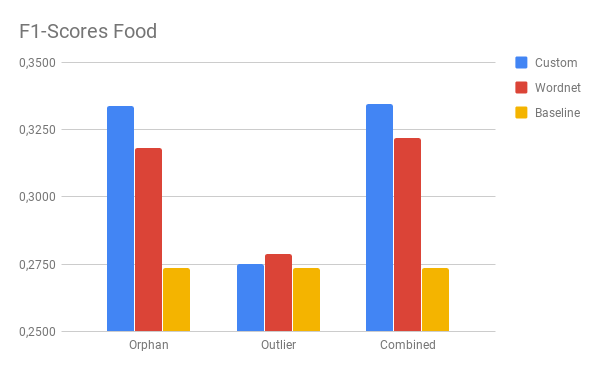
\includegraphics[width=1\textwidth]{images/F1-Scores_Food.png}
	\end{subfigure}
	\begin{subfigure}{0.45 \textwidth}
		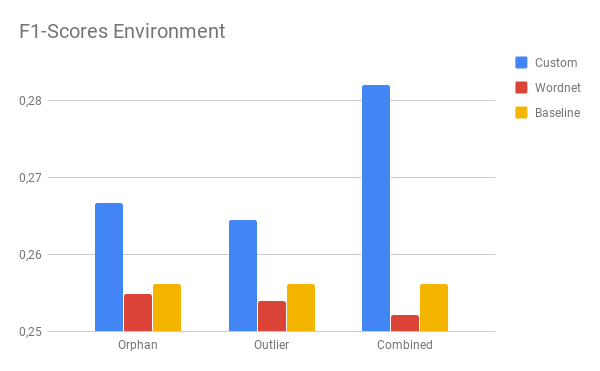
\includegraphics[width=1\textwidth]{images/F1-Scores_Environment.png}
	\end{subfigure}
	\caption{Contribution of outlier identification and orphan insertion to the total score for the food and environment domain}
	\label{contribution}
\end{figure}
\end{comment}

\paragraph{Ablation study} For this ablation study we analyze the scores when either outliers are removed or when orphans are connected to the taxonomy. Table \ref{results_abb} shows the respective scores as well as the actual score when both methods are combined. We can see that the food domain mostly benefits from the orphan insertion step, possibly since the food domain has the highest amount of unconnected nodes. However, both algorithms improved the taxonomy almost to an equal degree when applied to the environment domain. We further notice, that the algorithms appears to be complementary to each other as the separate improvements basically sum up, when combined. They are partly even higher than the sum, since identified outliers possibly create new orphans which are considered for the orphan insertion.

\begin{table*}[!htbp]
	\centering
	\resizebox{\textwidth}{!}{
		\begin{tabular}{*{5}{p{3cm}}}
			\toprule
			Domain & Method & Orphan & Outlier & Final\\
			\toprule
			Environment & Baseline & --- & ---& 25.62\\
			Environment & Poincaré Wordnet & 25.49 & 25.40 & 25.22\\
			Environment & Poincaré Custom & 26.67 & 26.65 & 28.21\\
			\midrule
			Science & Baseline & --- & ---& 36.63\\
			Science& Poincaré Wordnet & 39.49 & 37.80 & 40.58\\
			Science & Poincaré Custom & 39.86 & 37.13 & 41.69\\
			\midrule
			Food & Baseline & --- & ---& 27.36\\
			Food & Poincaré Wordnet & 31.83 & 27.90 & 32.18\\
			Food & Poincaré Custom & 33.37 & 27.52 & 33.47\\
			\midrule
			\bottomrule
		\end{tabular}}
		\caption{
			F$_1$ Scores with removed outliers or inserted orphans. Furthermore, the scores of both methods and the baseline for each Domain are shown. The final scores slightly differ from Table \ref{results_domains} as the last two sub-steps of Step \ref{Improved_Taxonomy} have not been applied.}
		\label{results_abb}
	\end{table*}
	
	
\paragraph{Comparison to Wordnet's Poincaré and Word2Vec}
The results of word2vec embeddings were sub-par. The interpretation of word similarity as co-hyponyms for our refinement method does not appear to be appropriate. However, using word2vec as a means to detect hypernyms has shown to be rather unsuitable since \cite{levy2015supervised} observed that even more complicated methods such as the \emph{diff} model \citep{fu2014learning, wang2017short}  do not actually learn a relation between two terms - they rather learn the independent attribute of a term to be a so called \emph{prototypical hypernym}. This information however, does not appear to be suitable for a taxonomy refinement method, since the identification of wrong relationships within the taxonomy and the attachment of new nodes needs to take the relationship between two terms of the taxonomy into account. Based on the results we achieved by using Poincaré embeddings, we hypothesize that their attributes result in a system that learns is-a relationships between terms by taking both words into account.
The Wordnet embeddings only beat the taxonomy-specific embeddings regarding the precision score for the food domain. In every other aspect the custom embeddings outperform Wordnet by a substantial margin.
Poincaré embeddings that are trained on Wordnet's hypernym relations are naturally more accurate. This can be seen in Table \ref{results_abb} for the step which removes outliers. The results of Wordnet are higher on average and appear to not be as much affected by different number of clusters as shown in Figure \ref{outlier_clusters}. However, the advantage of the custom embeddings enfold for the orphan insertion step, as seen in Table \ref{results_abb}. Most orphans either occur rarely or they are complex compounds like \emph{thermal discharge} and \emph{protection of plant life}. Table \ref{occurence of orphans} shows for each domain and embedding the number of orphans that were recognized and connected to the taxonomy. For two of three domains, the taxonomy-specific embeddings recognize almost two times the amount of terms.

\begin{table}[!htbp]
	\begin{tabular}{*{4}{p{1.4cm}}}
		\toprule
		Domain & Word2Vec & Wordnet & Custom \\
		\toprule
		Env. &58 & 18& 35\\
		Science &69 & 31 & 33\\
		Food & 257 & 147& 257 \\
		\bottomrule
	\end{tabular}
	\caption{
		Number of orphans of the baseline taxonomy that were reattached by using different embeddings
	}
	\label{occurence of orphans}
\end{table}

\paragraph{K-means as a selection method}
An important hyperparameter for the refinement method is the number of clusters $k$ for the k-means algorithm. As stated at the beginning, the pipeline was created with the idea in mind to be solely driven on the basis of raw text processing, since it makes the method more flexible and applicable to a variety of domains and languages. We thus avoided the use of supervised approaches, since they would require annotated data.
To use a static threshold also appeared unsuitable, since the distance and/or the ranks between entities of a taxonomy shifts with the size and structure of the taxonomy. A simple clustering technique such as k-means seems to be more suitable. The relevance of a selection method is much more important for the outlier removal than for the orphan insertion step. Figure \ref{outlier_clusters} shows the F$_1$-Scores for both Poincaré embeddings for varying cluster number $k$ as well as the baseline score. With exception of the food domain, the score increases mostly for any number of clusters, although a small $k$ appears to be more effective. As a general rule we observe that a bigger $k$ results in more removed relationships. This is most likely due to the main cluster becoming smaller with greater $k$ because the granularity increases. As seen in Figure \ref{precision_score}, which plots the recall and precision scores with increasing $k$ for the custom Poincaré embeddings, the precision only increases for small $k$, while the recall further decreases. That observation is reasonable as a smaller $k$ creates less but more confident identifications of outliers, as their rank deviation from the mean is most likely larger.
\begin{figure}[H]
	\begin{subfigure}{0.50 \textwidth}
		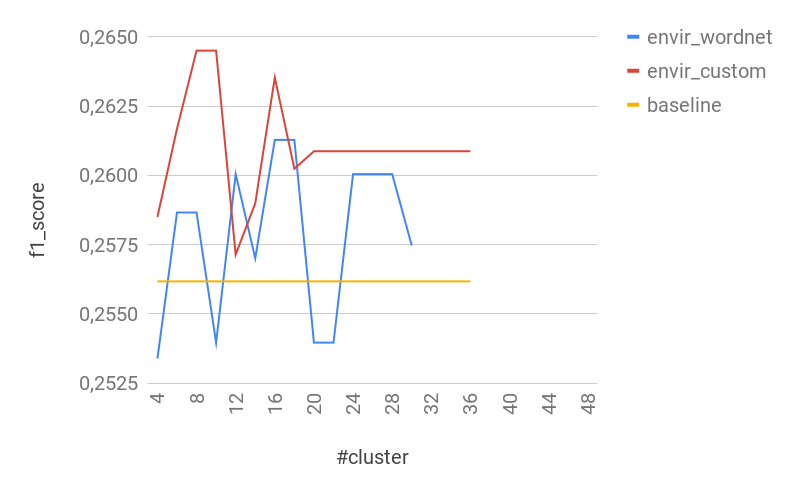
\includegraphics[width=1\textwidth]{images/environment_outlier.png}
		\caption{F$_1$ scores for environment}
	\end{subfigure}
	\begin{subfigure}{0.50 \textwidth}
		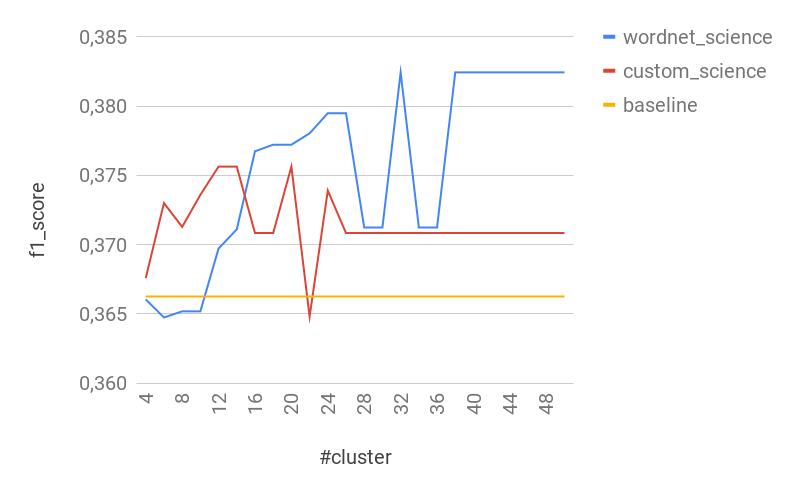
\includegraphics[width=1\textwidth]{images/science_outlier.png}
		\caption{F$_1$ scores for science}
	\end{subfigure}
	\begin{subfigure}{0.50 \textwidth}
		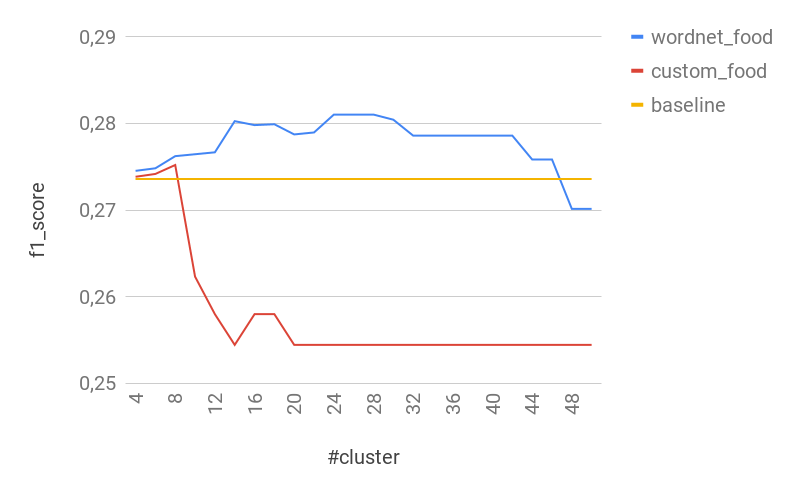
\includegraphics[width=1\textwidth]{images/food_outlier.png}
		\caption{F$_1$ scores for food}
	\end{subfigure}
	\begin{subfigure}{0.50 \textwidth}
		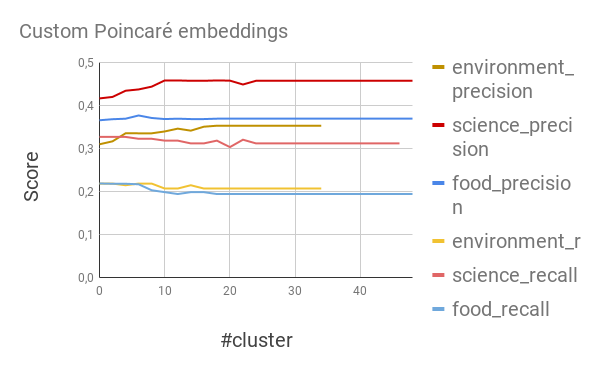
\includegraphics[width=1\textwidth]{images/Custom_Poincare_embeddings.png}
		\caption{Precision and recall scores for custom Poincaré embeddings}
		\label{precision_score}
	\end{subfigure}
	\caption{Scores of taxonomy with removed outliers for different number of clusters $k$.}
	\label{outlier_clusters}
\end{figure}


	

\section{Conclusion}

This work demonstrated a pipeline for improving an existing taxonomy through the use of distributional semantics, in particular Poincaré embeddings. They showed to be able to identify wrong hypernym relationships and add correct ones to the existing taxonomy so that the overall quality of the taxonomy improves. Poincaré embeddings outperformed the word2vec model significantly in the applied method. We further showed that the use of Poincaré embeddings trained on relationships, that were extracted on basis of a specific domain by raw text processing, are superior to ones trained on Wordnet. This rather simple use of Poincaré embeddings already leads to substantial improvements, so that additional applications and research of Poincaré embeddings is encouraged. Furthermore, we plan to apply the method to other languages to ensure its non-restrictive applicability. Based on the results of this experiment it would be highly interesting to further investigate, whether Poincaré embeddings address the raised concerns regarding word2vec embeddings, as a means for recognizing lexical inference relations.

\newpage




\bibliographystyle{apalike}
\bibliography{bibliography.bib}


\newpage
\appendix
\section*{Appendix}

\setcounter{table}{0}
\renewcommand{\thetable}{A\arabic{table}}

\begin{table}[!htbp]
	\begin{tabular}{*{2}{p{3.5cm}}}
		Parameter & Value \\
		\toprule
		Noisy relationships common & 27,612,520 \\
		Noisy relationships food & 11,109\\
		Noisy relationships science & 1,514\\
		Noisy relationships environment & 863\\
		$T_{f}$ common & 5 \\
		$T_{f}$ domain & 3 \\
		Cleaned relationships $|R|$ & 3102 \\
		Poincaré dim & 50 \\
		Poincaré epochs & 400 \\
		\midrule
		Word2vec corpus size & 3.1GB \\
		Word2vec dim & 300 \\
		Word2vec min\_count & 5 \\
		Word2vec epochs & 30 \\
		\midrule
		$k_{word2vec}$ & 3, 6 (orphan, outlier)\\ 
		$k_{wordnet}$ & 2, 20 (orphan, outlier)\\
		$k_{custom}$ & 2, 6 (orphan, outlier)\\
	\end{tabular}
	\caption{
		Parameters, settings and attributes of corpora, embeddings and clusters for different domains. The selected $k$ for each embedding is kept the same for all domains of the shared task.
	}
	\label{hyperparameters}
\end{table}


\end{document}

